\documentclass{standalone}

\begin{document}

% https://victorzhou.com/blog/intro-to-cnns-part-1/
% https://towardsdatascience.com/a-comprehensive-guide-to-convolutional-neural-networks-the-eli5-way-3bd2b1164a53
% https://ujjwalkarn.me/2016/08/11/intuitive-explanation-convnets/

\section[Convolution function]{Convolution function}\label{NN:convolutional}

A big revolution into the Neural Network research field was given by the introduction of the convolution functions.
Convolutional Neural Network (CNN) are particularly designed for image analysis.
Convolution is the mathematical integration of two functions in which the second one is translated by a given value:

$$
(f * g)(t) = \int_{-\infty}^{+\infty} f(\tau)g(t - \tau)d\tau
$$


In signal processing this operation is also called \emph{crossing correlation} ad it is equivalent to the \emph{autocorrelation} function computed in a given point.
In image processing the first function is represented by the image $I$ and the second one is a kernel $k$ (or filter) which shifts along the image.
In this case we will have a 2D discrete version of the formula given by:

$$
C = k * I
$$

$$
C[i, j] = \sum_{u=-N}^{N} \sum_{v=-M}^{M} k[u, v] \cdot I[i - u, j - v]
$$

where $C[i, j]$ is the pixel value of the resulting image and $N, M$ are kernel dimensions.

The use of CNN in modern image analysis applications can be traced back to multiple causes.
First of all the image dimensions are increasingly bigger and thus the number of variables/features, i.e pixels, is often too big to manage with standard DNN\footnote{
  If we consider a simple image $224\times224$ with $3$ color channels we obtain a set of $150'528$ features.
  A classical DNN layer with this input size should have $1024$ nodes for a total of more than $150$ million weights to tune.
}.
Moreover if we consider detection problems, i.e the problem of detecting a set of features (or an object) inside a larger pattern, we want a system ables to recognize the object regardless of where it appears into the input.
In other words, we want that our model would be independent by simple translations.

Both the above problems can overcome by CNN models using a small kernel, i.e weight mask, which maps the full input.
A CNN is able to successfully capture the spatial and temporal dependencies in an signal through the application of relevant filters.

The main parameter of this function are so given by the input dimensions and the filter/kernel dimensions, i.e the number of weight which we have to tune during the training.
This is the basic idea behind the convolution function but in many cases (especially in modern deep learning neural network) we can sophisticate it playing with the possible movements of the filter mask.
In particular, aside the kernel mask-size, we can also force the filter to jump along the image, i.e a discontinuous movement of the filter excluding some pixels.
This parameter, called \textsf{stride}, defines the number of pixels to jump and it is often used to reduce further the output dimensions.

Given this theoretical background we can implement the convolution function in many different ways, using different mathematical approaches: a study on the computational efficiency will tell us which is the best approach to choose.
The first (naive) approach is to use a brute force technique and implement the direct evaluation of the convolution functions as described above.
This version is certainly the easier to implement but its computational performances are so worst than for sake of brevity we excluded it from our tests\footnote{
  Compared to the other implementations the direct (brute force) convolution algorithm exceeds the computational time of order of magnitudes.
  For this reason it is not taken into account during our tests.
  A possible implementation in C++ is however provided into the \href{https://github.com/Nico-Curti/Byron/blob/master/utility/winograd_test.cpp}{Byron library}.
}.


\begin{center}
\begin{figure}[htbp]
\centering
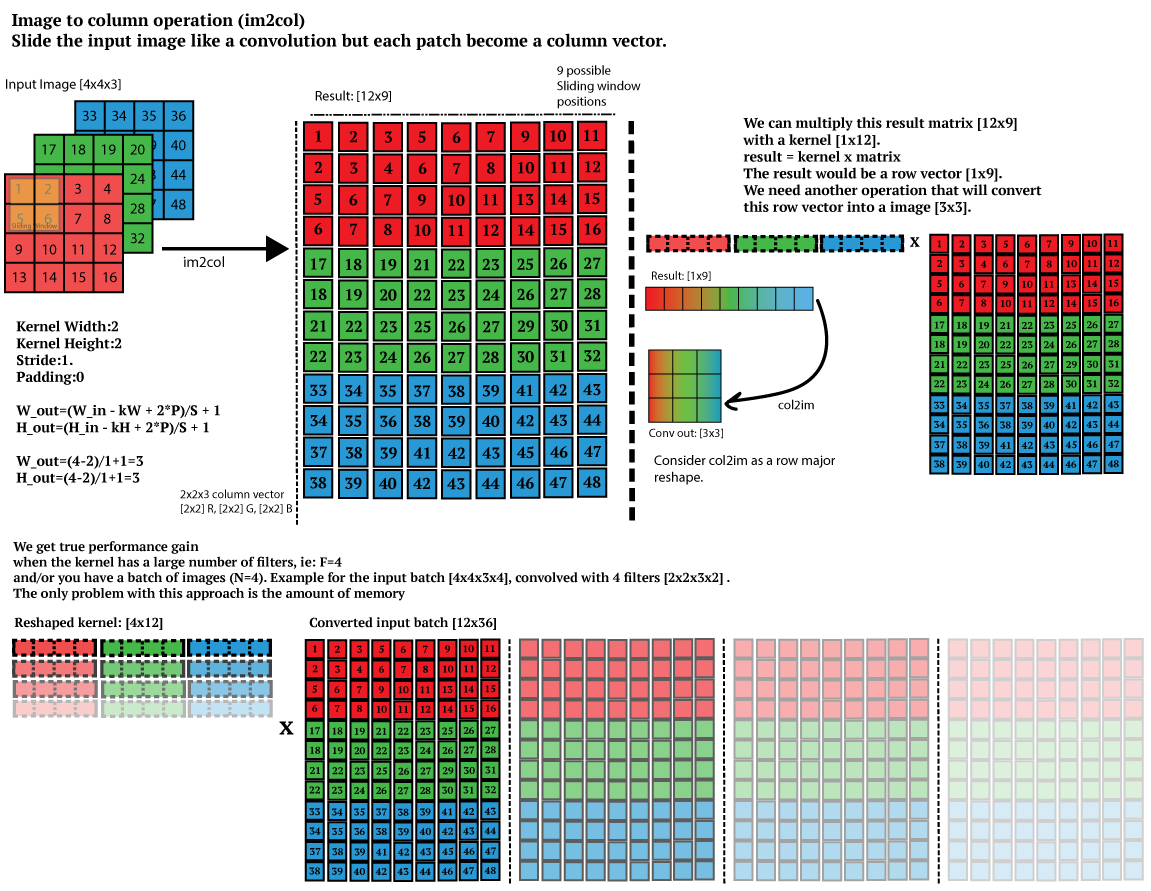
\includegraphics[width=0.85\textwidth]{im2col.png}
\caption{\textsf{im2col} algorithm scheme using a $2\times2$ filter on a image with 3 channels.
At the end of the \textsf{im2col} algorithm the GEMM is performed between weights and input image.
}
\label{fig:im2col}
\end{figure}
\end{center}


Taking into account what we have learned from the DNN models, we can re-formulate our problem using an efficient manipulation of the involved matrices to optimize the GEMM algorithm.
A direct convolution on an image of size ($W\times H\times C$) using a kernel mask of dimensions ($k \times k$) requires $O(WHCk^2)$ operations and thus many matrix products.
We can re-arrange the involved data to optimize this computation and thus evaluate a single matrix product: this re-arrangement is called \textsf{im2col} (or \textsf{im2row}) algorithm.
The algorithm is just a simple transformation which flats the original input into a bigger matrix where each column carries all the elements which have to be multiplied for the filter mask into a single step\footnote{
  We work under the assumption that the weights matrix is already a flatten array and thus each row of the weights matrix represents the full mask.
}.
In this way we can immediately apply our GEMM algorithm on the full image.
In Fig.~\ref{fig:im2col} the main scheme of this algorithm is reported.
This kind of algorithm certainly optimize the computation efficiency of the GEMM product but in payback we have to store a lot of memory for the input re-organization.

Using the mathematical theory behind the problem a third idea can arise using the well known Convolution Theorem: the Fourier transformation of our functions (that in this case are given by the input image and the weights kernel) can be reinterpreted into a simple matrix product in the frequency space.
This is certainly the most \quotes{physical} approach to solve this problem and probably the easier one since the Fourier transformation is a well-known optimized algorithm and many efficient implementations are already provided in literature.
One of the most efficient one is provided by the FFTW (\emph{Fast Fourier Transform in the West}) library~\cite{FFTW05}: the FFTW3 is an open source C subroutine library for computing the discrete Fourier transform (DFT) in multiple dimensions without constrains in input sizes or data types.
The library is not only accurate in the computation but it also provide an efficient parallel version for multi-threading applications.

A further implementation kind is given by linear algebra considerations (very closed to numerical considerations) and it is called Coppersmith-Winograd algorithm.
This algorithm was designed to optimize the matrix product and in particular to reduce the computational cost of its operations.
Suppose we have an input image given by just 4 elements and a filter mask with size equal to 3:

$$
\mbox{img} = \left[\begin{array}{cccc} d0 & d1 & d2 & d3 \end{array}\right] \quad\quad \mbox{weights} = \left[\begin{array}{ccc} g0 & g1 & g2 \end{array}\right]
$$
\\
we can now using the told above \textsf{im2col} algorithm and thus reshape our input image and weights into

$$
\mbox{img} = \left[
\begin{array}{ccc}
d0 & d1 & d2 \\
d1 & d2 & d3
\end{array}
\right],
\quad\quad
\mbox{weights} = \left[
\begin{array}{c}
g0 \\
g1 \\
g2
\end{array}
\right]
$$
\\
given this data we can simply compute the output as the matrix product of this two matrices.
The Winograd algorithm rewrites this computation as follow:

$$
\mbox{output} = \left[
\begin{array}{ccc}
d0 & d1 & d2 \\
d1 & d2 & d3
\end{array}
\right]
\left[
\begin{array}{c}
g0 \\
g1 \\
g2
\end{array}
\right] = \left[
\begin{array}{c}
m1 + m2 + m3 \\
m2 - m3 - m4
\end{array}
\right]
$$
\\
where

$$
m1 = (d0 - d2)g0\quad\quad m2 = (d1 + d2)\frac{g0 + g1 + g2}{2}
$$
$$
m4 = (d1 - d3)g2\quad\quad m3 = (d2 - d1)\frac{g0 - g1 + g2}{2}
$$
\\
where we can easily notice that the two fractions in $m2$ and $m3$ involve only weight quantities and thus they have to be computed only one time for each filter (at each step).
Moreover we have to manage 4 ADD and 4 MUL operations to calculate the $m_i$ quantities and 4 other ADD to compute the result.
In doing normal matrix products we have to do 6 MUL operations instead of 4.
This is reducing computationally expensive MUL operations by a factor of 1.5x which is very significant\footnote{
  A multiplication takes 7 clock cycles in a normal CPU while an add takes only 3 clock cycles.
}.
In this simple example we use a so-called $F(4, 3)$, i.e image of size 4 and kernel of size 3 which gives us 2 convolutions.
More general formulations are $F(m\times m, r \times r)$ and if we use an image of size $4\times4$ and a kernel of size $3\times3$ we can compare the 16 MULs of the Winograd algorithm against the 36 MULs which are required by the normal matrix product (2.25x).
The Winograd efficiency was widely proofed for Convolutional network models, especially when the kernel size is small.
In our Byron library we provide its implementation for kernel sizes equal to 3 since the numerical generalization is not straight-forward\footnote{
  We would also highlight that this formulation is valid only if we consider unitary strides.
}.

To test which algorithm could be more appropriated for Neural Network models we tested their computational time efficiency on different random images.
The tests were performed on a classical bioinformatics server (128~GB RAM memory and 2 CPU E5-2620, with 8 cores each) and we considered only kernel sizes equal to 3 (Winograd constrain) varying the input dimensions and the number of filters.
In Fig.~\ref{fig:winograd_timing} we show the result of our simulations using the \textsf{im2col} values as reference\footnote{
  The \textsf{im2col} algorithm can be found in the major part of Neural Network library and it is also the only convolution function implemented in the \textsf{darknet} library, which is a sort of reference for our work.
}.

\begin{figure}[htbp]
\centering
\def\svgwidth{0.8\textwidth}
\input{./img/winograd_timing.pdf_tex}
\caption{Time performances of different convolution algorithms: \textsf{im2col} (orange, reference), \textsf{FFTW3} (green, fast Fourier transformation using the FFTW3 library) and \textsf{Winograd} (blue).
The values are normalized according to the \textsf{im2col} results since it is the most common convolution algorithm.
The tests were performed on different input sizes (width/height), keeping fixed the number of channels and the number of filters.
The tests were performed using a C++ implementation of the three methods.
}
\label{fig:winograd_timing}
\end{figure}

In all our simulations we found a visible speedup using the \textsf{Winograd} algorithm against the other two algorithms: for small dimensions we obtain more than 5x against the \textsf{im2col} and 25x against the \textsf{fftw} implementation.
The worst algorithm is certainly the \textsf{fftw} one which, despite the efficient FFTW3 parallel-library, is always more than 5 times slower than the reference.
However, it is interesting notice how the \textsf{fftw} implementation is able to reach the best performances when the dimensions are proportional to powers of 2, as expected from the mathematical theory behind the Discrete Fourier Transformation.

We can conclude that the \textsf{Winograd} algorithm is certainly the best choice when we have to perform a 2D convolution.
The payback of this method is given by the rigid constrains related to the mask sizes and strides: when it is possible it remains the best solution but in all the other cases the \textsf{im2col} implementation is a relatively good alternative.
The efficiency of Byron library follows the efficiency of the \textsf{Winograd} algorithm since the major part of layers in modern deep learning Neural Network models are Convolutional layers with size equal to 3 and unitary stride.

%https://victorzhou.com/blog/intro-to-cnns-part-1/


\end{document}
